\documentclass{standalone}
\usepackage{tikz}
\usepackage{ctex,siunitx}
\setCJKmainfont{Noto Serif CJK SC}
\usepackage{tkz-euclide}
\usepackage{amsmath}
\usetikzlibrary{patterns, calc,3d}
\usetikzlibrary {decorations.pathmorphing,decorations.pathreplacing,decorations.shapes}
\begin{document}
\small
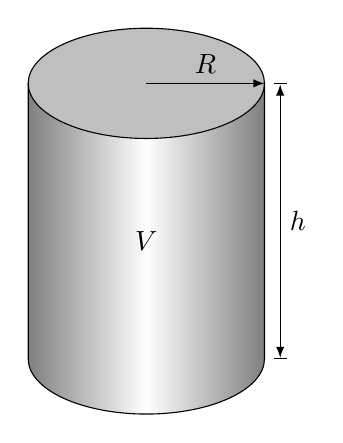
\begin{tikzpicture}[>=latex,scale=1.0]
  \draw[left color=gray,right color=gray,middle color=white](-1.5,0)arc(180:360:1.5 and 0.7)--(1.5,3.5)--(-1.5,3.5)--cycle;
  \draw[fill=lightgray](0,3.5)ellipse(1.5 and 0.7);
  \node at (0,1.5){$V$};
  \draw[->](0,3.5)--(1.5,3.5)node[midway,above]{$R$};
  \draw[|<->|](1.7,0)--(1.7,3.5)node[midway,right]{$h$};
\end{tikzpicture}
\end{document}